The elastically-scattered electrons provided the clearest point in extracting the energy resolution of the Ecal at the beam energy. Using WAB particles, electrons and photons, the energy resolution of the Ecal was fully characterized in terms of energy and position relative to the edges.\\
\indent To study the energy resolution in the fiducial region of the Ecal, all electrons were matched to tracks, and the track position extrapolated to the incident face of the Ecal was used to determine the electron's vertical distance relative to the beam gap edge. For elastically-scattered electrons, one track-matched electron is used. For WAB electrons, the photon cluster was required to be at least 10~mm from the Ecal edges as this way, the reconstructed photon energy is reliable. By selecting WAB events where the energy difference between the two particles is less than 100~MeV, the resolution of the energy sum peak was fitted to extract the resolution. The resolution was extracted according to Equation~\eqref{eq:eResExtract}.

\begin{equation}
	\label{eq:eResExtract}
	\sigma_{E_{\gamma}+E_{e-}}^2 = \sigma_{e-}^2(E_{e-})+\sigma_{\gamma}^2(E_{\gamma})
\end{equation}

When both particles are in the fiducial region and are roughly equal in energy, then the energy resolution of the sum could be divided by $\sqrt{2}$ assuming that the energy resolution of both particles is the same. This same procedure was used to study the resolution when the particle energies were more asymmetric in energy in order to obtain the single particle energy resolution at various energies. \\
\indent The experimentally-obtained fiducial energy resolution agrees well with Monte Carlo but generally yields a slightly larger energy resolution across all energies (on the order of about 15$\%$). The energy resolution obtained in data is shown in Figure~\ref{Figure:eResData}.

\begin{figure}[H]
  \centering
      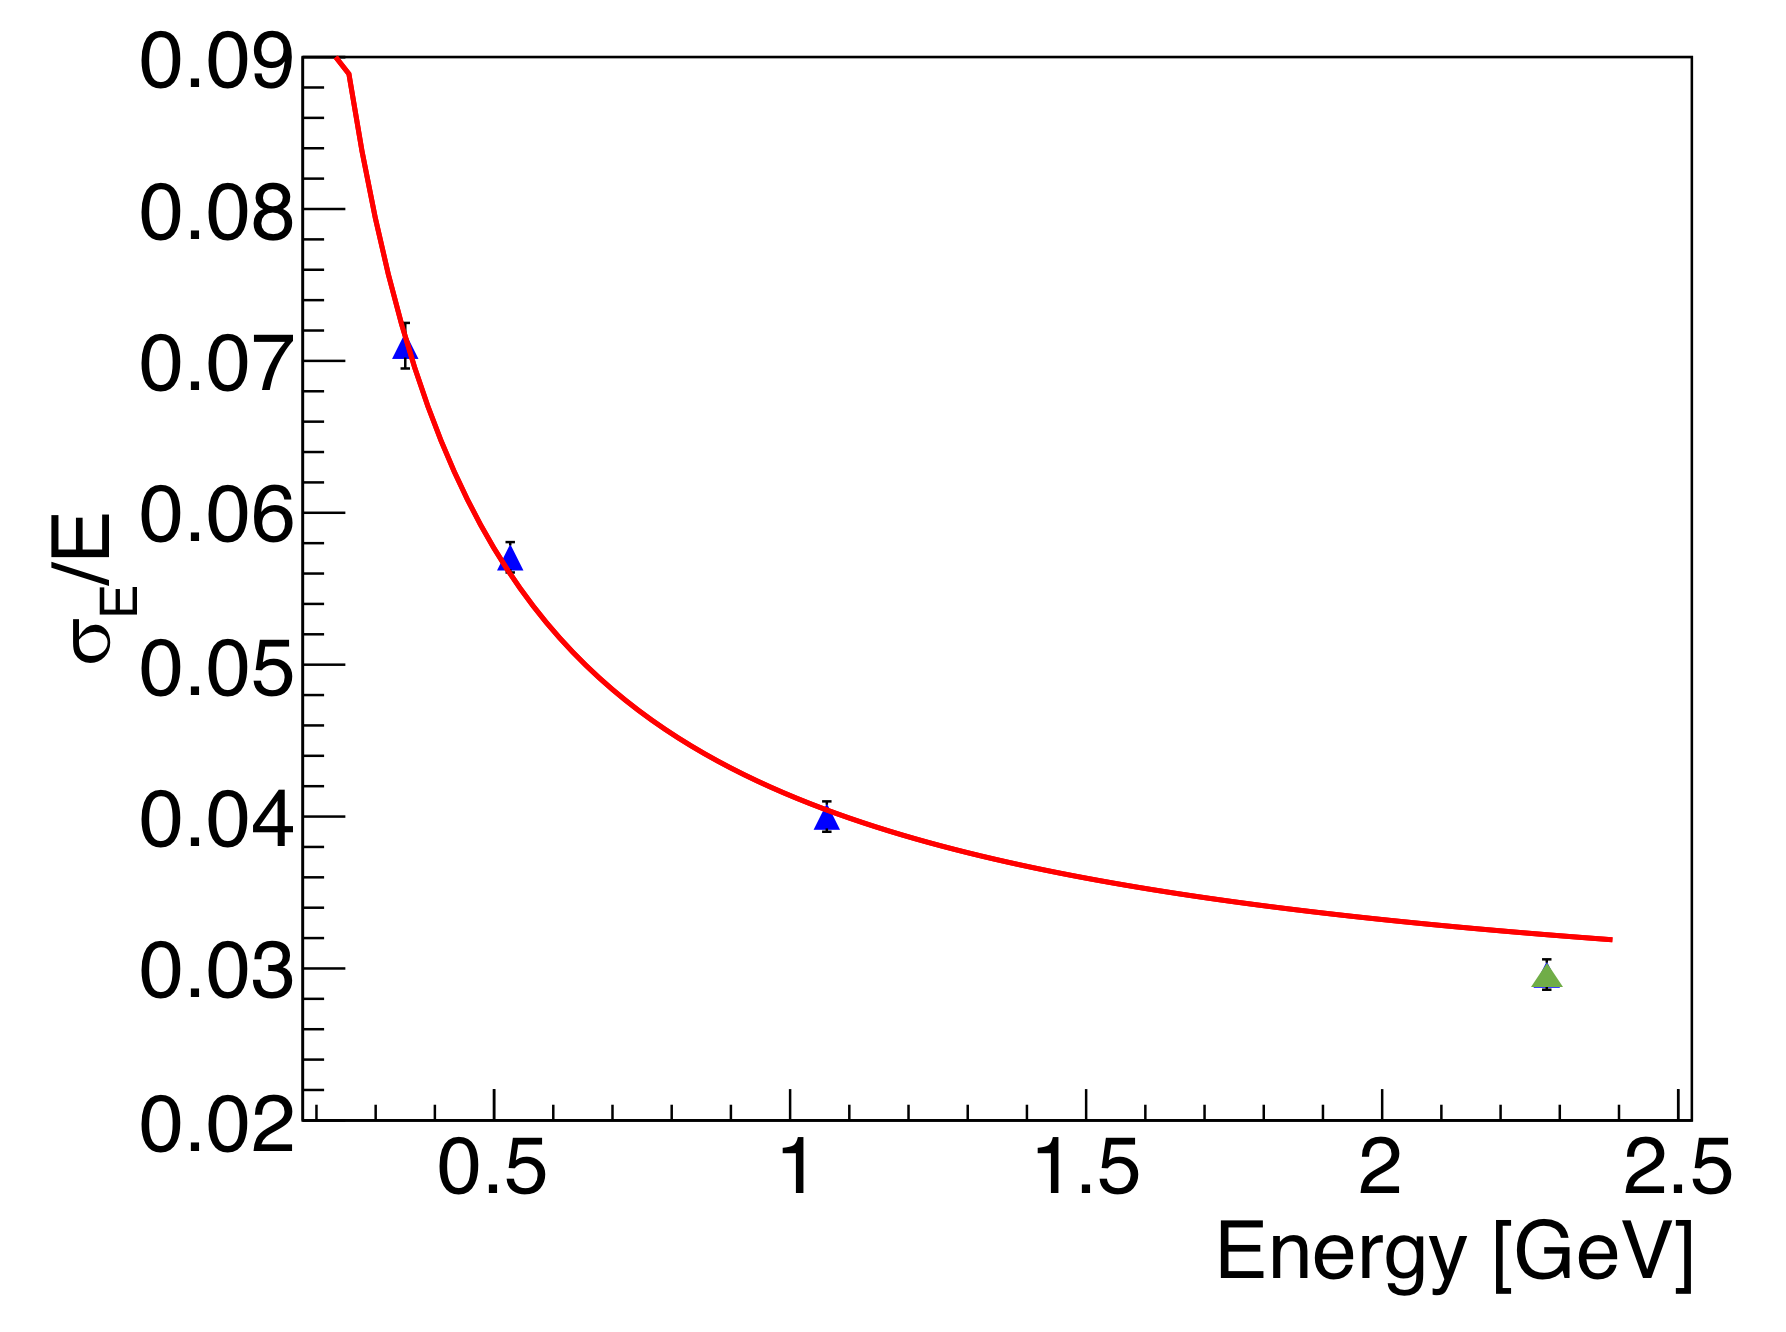
\includegraphics[width=0.9\textwidth]{pics/performance/eResData.png}
  \caption[Energy resolution of the Ecal found in data]{The blue points are derived from the 2015 running for the energy resolution of a single particle. The green point at approximately 2.3~GeV was determined from the elastic calibration of the 2016 data. The fitted energy resolution was determined from the 2015 data only, but it shown here extrapolated to the 2016 energy.}
  \label{Figure:eResData}
\end{figure}

The fit to the energy resolution in data is shown in Equation~\eqref{eq:eResData} and is fit to the blue points representative of the 2015 data in Figure~\ref{Figure:eResData}.

\begin{equation}
	\label{eq:eResData}
	\dfrac{\sigma_E}{E}(\%) = \dfrac{1.62}{E}\bigoplus\dfrac{2.87}{\sqrt{E}}\bigoplus2.5
\end{equation}

The first term in Equation~\eqref{eq:eResData} is generally attributed to the noise from the pre-amplifiers and is roughly consistent to that found in Monte Carlo. The second term is related to the statistical fluctuations of the shower containment and the APD gain. This term is larger than the term found in Monte Carlo but is still roughly consistent. The third term contains both the energy leakage out the back of the Ecal as well as the crystal-to-crystal inter-calibration error. This term is significantly higher than that derived in Monte Carlo, but is much closer to the term as found in data for the CLAS Inner Calorimeter. It's possible that this term is affected by the inability to calibrate several crystals along the outer edges of the calorimeter with elastics. \\
\indent The energy resolution as found in 2016 at 2.3~GeV (shown in green on Figure~\ref{Figure:eResData}) is slightly better than that predicted by the fit to the 2015 points. It is likely that the energy resolution of the Ecal improved overall in 2016 as compared to 2015 because the TDCs were removed, and the signal going into the FADCs was no longer split. 
